\subsection*{Exercice 1 -- Fonction mystère}
\textit{D'après ressources de C. Lambert.}
On donne la fonction suivante : 
\begin{py}
\begin{python}
def mystere(L):
    """
    Ceci est la fonction mystère, saurez-vous 
    trouver son but ?
    Entrée : 
        * L(list) : liste de nombres entiers
    ou réels
    Sortie : 
        * ??? 
    """
    n = len(L)
    if n==0 :
        return (None)
    elif n==1 :
        return (L[0])
    else :
        x = mystere(L[0:n-1])
        if x<=L[-1] :
            return (x)
        else : 
            return (L[-1])
\end{python}
\end{py}

\subparagraph{}
\textit{Sans coder la fonction, déterminer le résultat de l'instruction \textbf{print(mystere([14, 20, 3, 16]))} ? Vous pourrez représenter de façon graphique l'empilement et le dépilement de la pile d'exécution.}

\subparagraph{}
\textit{D'après vous quel est le but de cette fonction ?}

\subparagraph{}
\textit{Programmer la fonction et tester l'instruction précédente. Sur plusieurs exemples, vérifiez la conjecture faite à la question précédente.}


\subparagraph{}
\textit{Question subsidiaire. -- Montrer que la propriété suivante est une propriété d'invariance :\\
$\mathcal{P}(k)$ : l'algorithme retourne le plus petit élément de toute liste de taille $k$.}

\begin{rem}
\begin{itemize}
\item Il faudra montrer que l'algorithme se termine au moyen d'un variant de boucle. 
\item Il faudra montrer $\mathcal{P}$ par récurrence. 
\end{itemize}
\end{rem}
\ifprof
\begin{corrige}
Soit $L$ une liste de taille $n$. Alors $n$ est un variant de boucle car : 
\begin{itemize}
\item si $n=1$ ou $n=0$, l'algorithme se termine ;
\item si $n>1$ chaque appel récursif est réalisé avec l'argument $L[0:n-1]$, qui est de longueur $n-1$. Ainsi $n$ 
décrit une suite strictement décroissante, jusqu'à ce que $n=1$ (terminaison de l'algorithme). 
\end{itemize}

\vspace{.25cm}

Soit la propriété suivante : soit $L$ une liste de taille $k$. L'appel à la fonction mystère retourne le plus petit 
élément de $L$. Montrons-le par récurrence.

Pour une liste de longueur 0 ou 1, le résultat est immédiat.

%Soit une liste de 2 éléments. $x$ reçoit le premier élément de la liste. $x$ est comparé au second élément. Si $x$ est 
%inférieur au second élément, c'est donc le plus petit élément. $x$ est bien retourné. Sinon c'est bien le second 
%élément qui est retourné. 


Soit une liste de taille $k+1$.  Alors $x$ reçoit le résultat de \texttt{mystere(L[0:k])}. D'après la propriété, $x$ 
contient donc le plus petit élément de la liste \texttt{L[0:k]}. Ensuite $x$ est comparé à l'élément \texttt{L[k]}. Si 
$x$ est inférieur à cet élément, c'est donc le plus petit élément, et $x$ est bien retourné. Sinon c'est que l'élément 
\texttt{L[k]} est le plus petit de la liste. C'est bien celui qui est retourné. 

La propriété énoncée est donc bien héréditaire, et l'algorithme renvoie bien toujours le minimum de la liste entrée en 
argument.
\end{corrige}
\else
\fi

\subsection*{Exercice 2 -- Palindrome...}
\textit{D'après ressources de C. Lambert.}
\setcounter{subparagraph}{0}
On souhaite réaliser une fonction \texttt{miroir} dont le but est de retourner le <<miroir>> d'une chaîne de caractères. 
Par exemple le résultat de \texttt{miroir("miroir")} serait \textsl{''riorim''}.

\subparagraph{}
\textit{Programmer la fonction \texttt{miroir\_it} permettant de répondre au problème de manière itérative.}


\subparagraph{}
\textit{Programmer la fonction \texttt{miroir\_rec} permettant de répondre au problème de manière récursive.}


\subparagraph{}
\textit{Que renvoie la fonction si la chaîne de caractère est "Eh ! ça va la vache" ?}
 
 \subparagraph{}
\textit{Évaluer la complexité algorithmique de chacune des deux fonctions.}

 
\subsection*{Exercice 3 -- Suite de Fibonacci}
\textit{D'après ressources de C. Lambert.}

\setcounter{subparagraph}{0}
On définit la suite de Fibonacci de la façon suivante : 
$$
\forall n\in \mathbb{N}, \left\{ \begin{array}{l}
u_0 = 0, u_1 = 1 \\
u_{n+2} = u_{n} + u_{n+1}
\end{array}\right.
$$

\subparagraph{}
\textit{Définir la fonction \texttt{fibonacci\_it} permettant de calculer $u_n$ par une méthode itérative. Évaluer la 
complexité algorithmique de l'algorithme.}

\subparagraph{}
\textit{Définir la fonction \texttt{fibonacci\_rec} permettant de calculer $u_n$ par une méthode récursive << 
intuitive>>. Évaluer la complexité algorithmique de l'algorithme.}


\subparagraph{}
\textit{Observer comment passer du couple $(u_n,u_{n+1})$ au couple $(u_{n+1},u_{n+2})$. En déduire une autre méthode 
récursive pour calculer le n\ieme terme de la suite de Fibonacci. Évaluer la complexité algorithmique de l'algorithme.}


\section*{Exercice 4 -- Les tours de Hanoï}
\setcounter{subparagraph}{0}

On considère le problème suivant, connu sous le nom des \emph{tours de Hanoï}.

\begin{center}
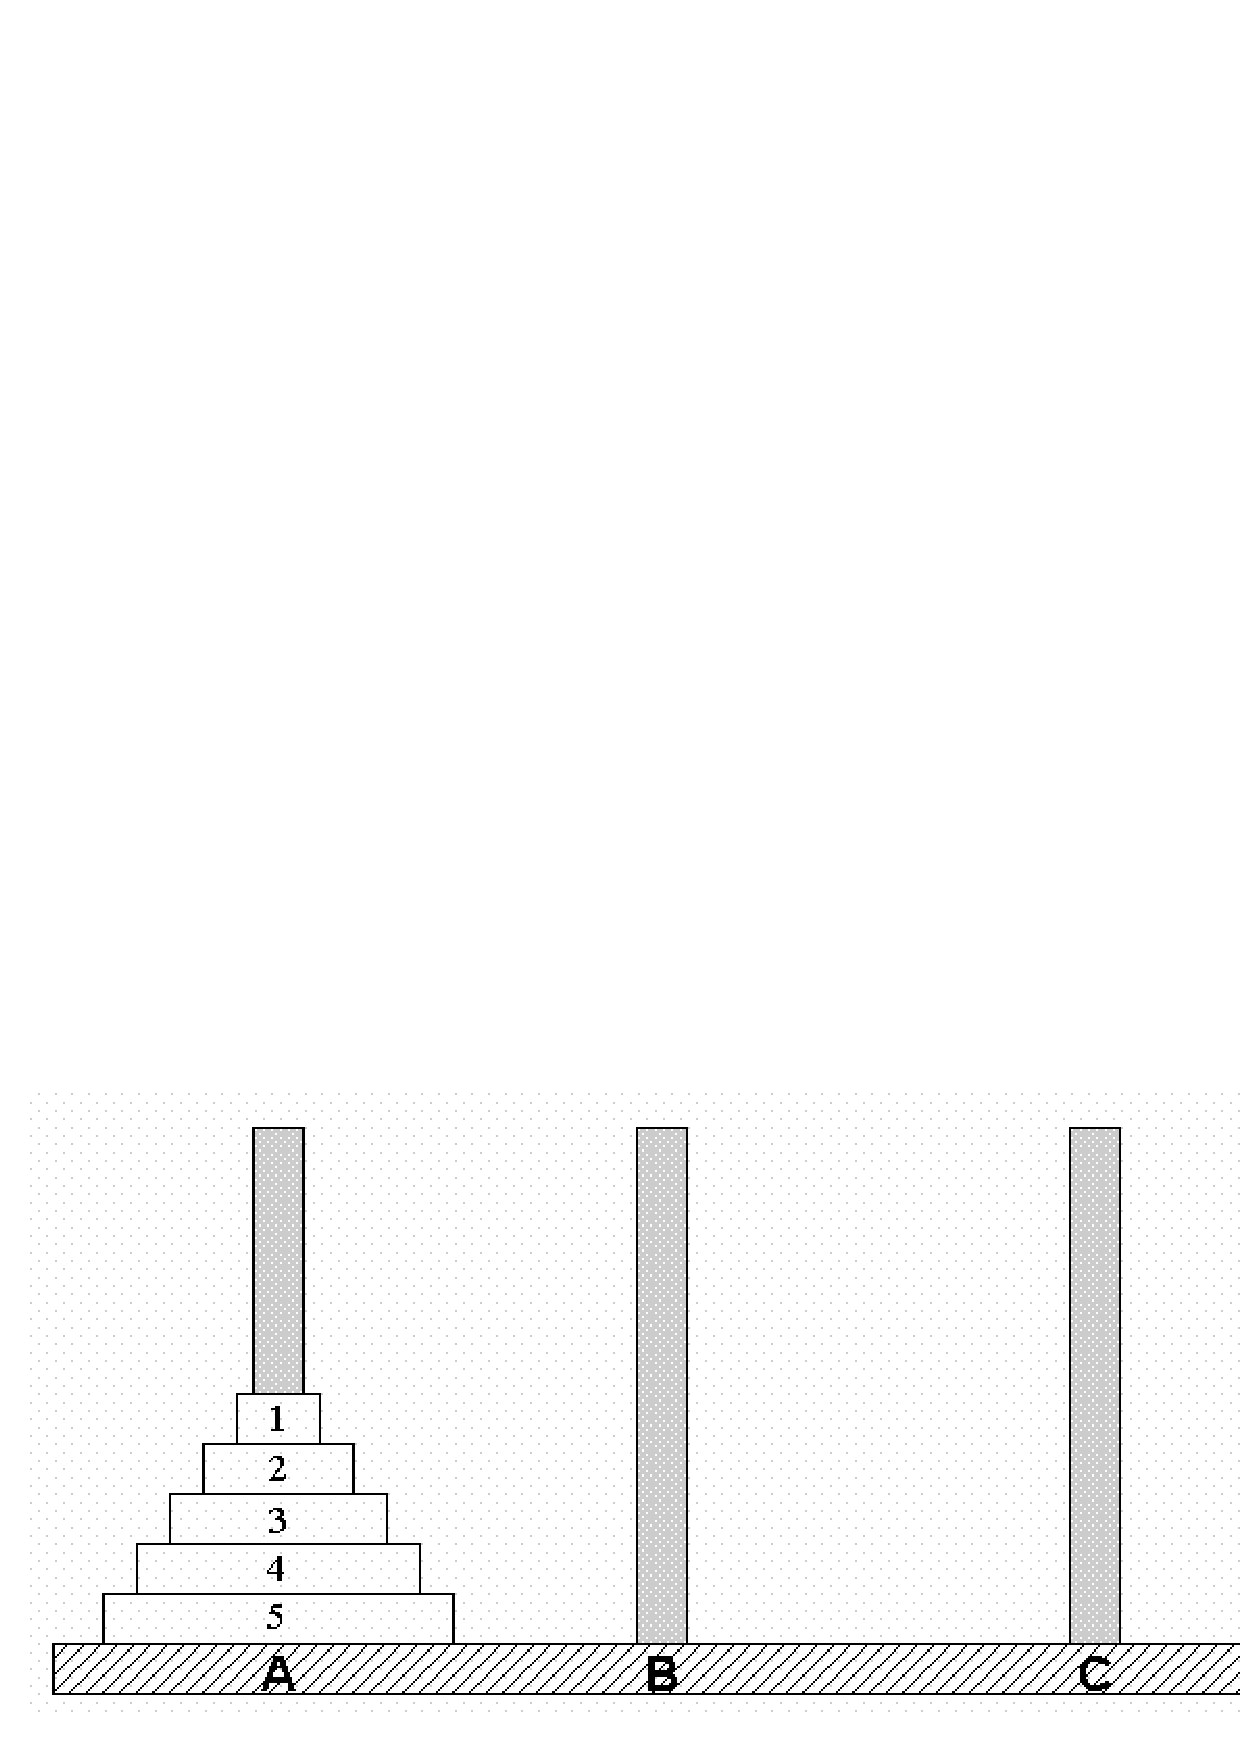
\includegraphics[scale=0.3]{images/hanoi.png}
\end{center}

On dispose de $n$ disques de diamètres tous différents, qui sont empilés sur un piquet $A$, par ordre croissant 
de 
diamètre, en les regardant de haut en bas. On dispose de deux autres piquets vides $B$ et $C$, et le but est de 
déplacer tous les disques sur le piquet $C$, en respectant quelques règles :
\begin{itemize}
\item on a le droit d'utiliser tous les piquets ;
\item à la fin, les disques doivent toujours être rangés par ordre croissant de diamètre, en les regardant de 
haut 
en bas ;
\item on ne peut déplacer les disques que un par un ;
\item on ne peut empiler un disque que sur un disque de diamètre inférieur.
\end{itemize}

\textit{Ce problème est très compliqué à résoudre de manière directe.\\
Il est par contre très simple à résoudre de manière récursive.}

\subparagraph{} 
\textit{Résoudre le problème pour $n=1$.}

\ifprof
\begin{corrige}
Trivial : on déplace le disque du piquet $A$ et on le place sur le piquet $C$.
\end{corrige}
\else
\fi

\subparagraph{} 
\textit{On suppose que l'on sait résoudre le problème pour $n-1$ disques. Donner alors une résolution du 
problème pour $n$ disques.}

\ifprof
\begin{corrige}
Si l'on sait transférer $n-1$ disques, il suffit de
transférer $n-1$ disques vers le piquet B, puis le $n$-ème disque vers le piquet C et enfin de transférer les $n-1$ 
disques du piquet B vers le piquet C.
\end{corrige}
\else
\fi

\subparagraph{} 
\textit{
Écrivez maintenant un programme \textbf{\underline{récursif}} résolvant ce problème. Il s'agit d'écrire 
un programme \texttt{hanoi} ayant quatre arguments $A$, $B$, $C$ et $n$ : 
\begin{itemize}
\item le premier, $A$, est le piquet sur lequel se trouvent les disques au départ ;
\item le second, $B$, est le piquet ``de transition'' ;
\item le troisième, $C$, est le piquet sur lequel on veut récupérer les disques à la fin ;
\item et enfin le quatrième et dernier argument, $n$, est le nombre de disques.
\end{itemize}}

\textit{On lui demande également d'afficher tous les déplacements effectués sous forme de chaînes : la chaîne 
\texttt{``a->b''} signifie par exemple que le disque du dessus du piquet $A$ est déplacé sur le piquet $B$. On 
utilisera le programme 
d'impression des déplacements suivant :\\}

\begin{py}
\begin{python}
def deplace (x, y) :
    print (x + ''->'' + y + ''\n'')
\end{python}
\end{py}

\textit{Attention : $A$, $B$, $C$, $x$ et $y$ sont ici de type \texttt{string}.\\}

\textit{Écrire le programme \texttt{hanoi}. Attention : il s'agit d'un programme récursif, qui va donc être très court 
! En 
aucun cas le programme en lui-même ne fait apparaître les opérations effectuées.}

\ifprof
\begin{corrige}

\begin{py}
\begin{python}
def hanoi (A, B, C, n) :
    if n == 1 :
	deplace (A,C)
    else :
	hanoi (A,C,B,n-1)
	hanoi (A,B,C,1)
	hanoi (B,A,C,n-1)
\end{python}
\end{py}

\end{corrige}
\else
\fi

\section*{Exercice 5 -- Faisons des Bulles}
\textit{ D'après les ressources de Mmes SEMBELY et VERDIER}
\setcounter{subparagraph}{0}

Les fractales sont des objets mathématiques fondés sur des figures géométriques se répétant à l'infini via un processus 
itératif.
\begin{center}
\textit{ "Une fractale est un objet irrégulier, dont l'irrégularité est la même à toutes les échelles et en tous les 
points"
\\
Adrien DOUADY - mathématicien français}
\end{center}
Ce type de structure se retrouve également dans la nature : architecture des côtes maritimes, ramifications nerveuses, 
nuages, galaxies ...
\\
Etant donné leur structure, il est très intéressant d'utiliser la récursivité pour visualiser des ensembles fractals.
\\
\subparagraph{}
\textit{Ecrire une fonction \texttt{cercle} d'arguments \texttt{x}, \texttt{y} et \texttt{r} qui trace le cercle de 
centre le point $A(x, y)$ et de rayon $r$ (supposé strictement positif).}

\subparagraph{}
\textit{Ecrire une fonction récursive \texttt{bubble} d'arguments \texttt{x}, \texttt{y}, \texttt{r} et \texttt{n}. Elle 
effectuera la construction pour un nombre \texttt{n} d'étapes en ayant pour figure de base le cercle de centre $A(x, y)$ 
et de rayon \texttt{r} (supposé strictement positif).}
\textit{À chaque étape, le rayon du cercle est divisé par 2.}
\begin{center}
\includegraphics[width=.65\linewidth]{images/fig_03}
% Le résultat des fonctions bubble1(4) et de bubble2(4).
\end{center}

\subparagraph{}
\textit{Ecrire une fonction récursive \texttt{bubbleComplet} d'arguments \texttt{x}, \texttt{y}, \texttt{r}, \texttt{n} 
et une chaîne de caractères \texttt{position}. Elle effectuera la construction ci-dessous pour un nombre \texttt{n} 
d'étapes en ayant pour figure de base le cercle de centre $A(x, y)$ et de rayon \texttt{r} (supposé strictement 
positif).}
\begin{center}
\includegraphics[width=.65\linewidth]{images/bulles}
% Le résultat des fonctions bubble1(4) et de bubble2(4).
\end{center}

\ifprof
\begin{corrige}
\begin{python}
### tracé d'un cercle
import matplotlib.pyplot as plt
import numpy as np

def cercle(x,y,r):
    """tracé d'un cercle de centre A(x,y) et de rayon r"""
    angles=np.linspace(0,2*np.pi,500)
    les_X=[x+r*np.cos(angle) for angle in angles]
    les_Y=[y+r*np.sin(angle) for angle in angles]
    plt.plot(les_X,les_Y)
    plt.axis("equal")
    plt.show()
    
def cerclesRec(x,y,r,n):
    """tracé des cercles à droite et en bas du cercle de centre A(x,y) et de rayon r"""
    cercle(x,y,r)
    if n>0:
        cerclesRec(x+1.5*r,y,r/2,n-1)
        cerclesRec(x,y-1.5*r,r/2,n-1)
        
def cerclesRec_2(x,y,r,n,position):
    """tracé des cercles autour du cercle de centre A(x,y) et de rayon r"""
    cercle(x,y,r)
    if n>0:
        if position=='centre':
            cerclesRec_2(x,y+1.5*r,r/2,n-1,'haut')
            cerclesRec_2(x-1.5*r,y,r/2,n-1,'gauche')
            cerclesRec_2(x+1.5*r,y,r/2,n-1,'droite')
            cerclesRec_2(x,y-1.5*r,r/2,n-1,'bas')
        if position=='droite':
            cerclesRec_2(x,y+1.5*r,r/2,n-1,'haut')
            cerclesRec_2(x+1.5*r,y,r/2,n-1,'droite')
            cerclesRec_2(x,y-1.5*r,r/2,n-1,'bas')
        if position=='bas':
            cerclesRec_2(x-1.5*r,y,r/2,n-1,'gauche')
            cerclesRec_2(x+1.5*r,y,r/2,n-1,'droite')
            cerclesRec_2(x,y-1.5*r,r/2,n-1,'bas')
        if position=='gauche':
            cerclesRec_2(x-1.5*r,y,r/2,n-1,'gauche')
            cerclesRec_2(x,y+1.5*r,r/2,n-1,'haut')
            cerclesRec_2(x,y-1.5*r,r/2,n-1,'bas')
        if position=='haut':
            cerclesRec_2(x-1.5*r,y,r/2,n-1,'gauche')
            cerclesRec_2(x+1.5*r,y,r/2,n-1,'droite')
            cerclesRec_2(x,y+1.5*r,r/2,n-1,'haut')
\end{python}
\end{corrige}
\else
\fi






